Để đánh giá tính thực tiễn của cấu trúc danh mục đã được tối ưu hóa bằng t-Student Copula, nghiên cứu tiến hành mô phỏng quỹ đạo tài sản (Asset Paths) trong chu kỳ 1 năm (tương đương 252 ngày giao dịch) dựa trên 10.000 kịch bản Monte Carlo. Giả định giá trị vốn gốc ban đầu được chuẩn hóa là 1.0.

\begin{figure}[H]
    \centering
    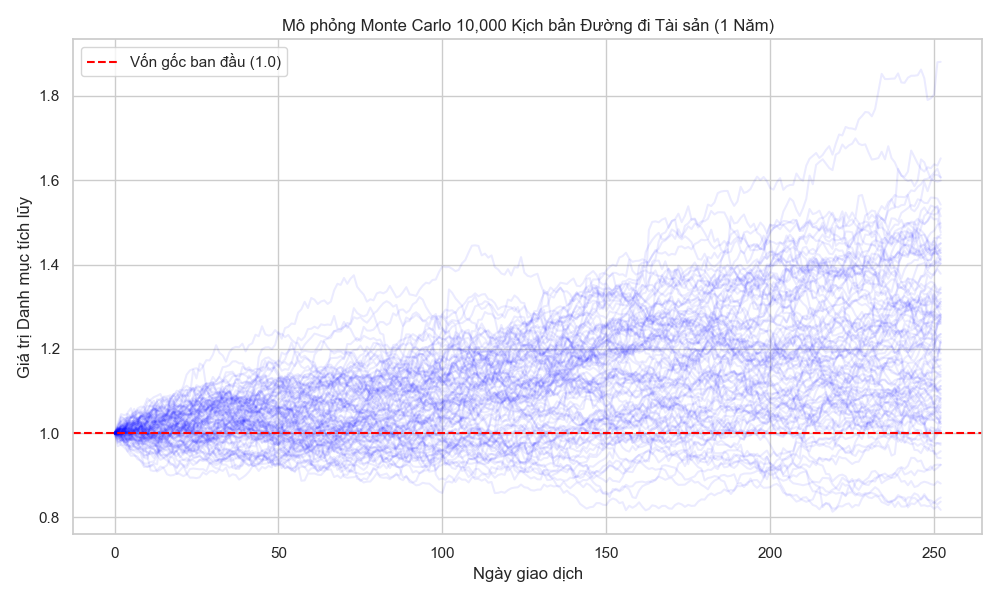
\includegraphics[width=0.9\textwidth]{monte_carlo_paths.png}
    \caption{Mô phỏng Monte Carlo 10.000 kịch bản quỹ đạo tài sản tích lũy trong 1 năm}
    \label{fig:mc_paths}
\end{figure}

Hình \ref{fig:mc_paths} minh họa quá trình tiến hóa của giá trị danh mục qua thời gian. Mặc dù có sự phân tán rộng do tính biến động tự nhiên của các cổ phiếu công nghệ, xu hướng chung của đám mây điểm cho thấy sự tăng trưởng tích cực, phần lớn các quỹ đạo đều nằm trên mức vốn gốc ban đầu (đường gạch đứt màu đỏ). Để lượng hóa chính xác hơn rủi ro và lợi nhuận tại thời điểm đáo hạn (ngày giao dịch thứ 252), phân phối giá trị tài sản cuối kỳ được trình bày tại Hình \ref{fig:mc_terminal}.

\begin{figure}[H]
    \centering
    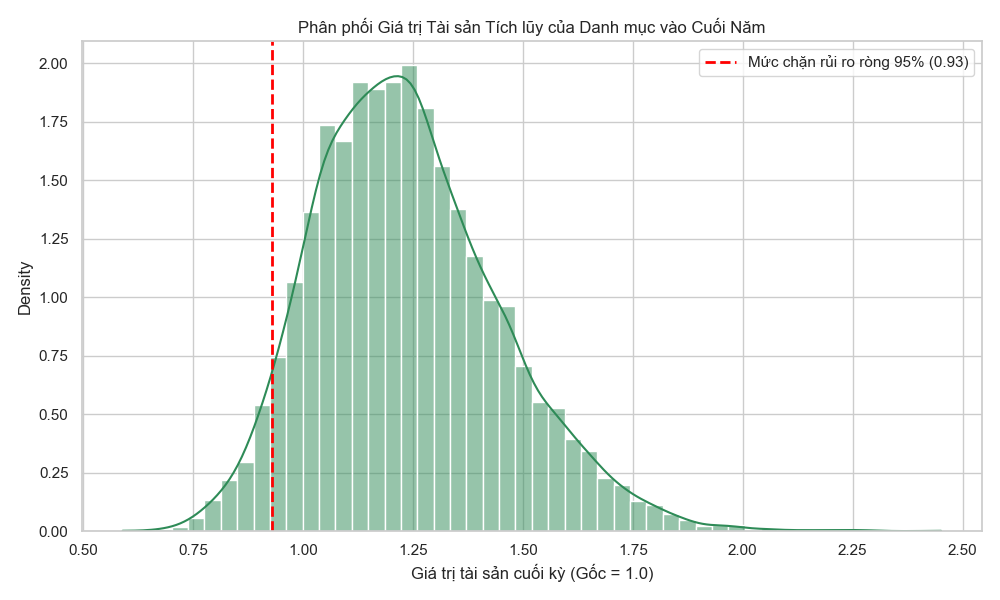
\includegraphics[width=0.85\textwidth]{final_asset_distribution.png}
    \caption{Phân phối giá trị tài sản tích lũy của danh mục vào cuối năm}
    \label{fig:mc_terminal}
\end{figure}

\begin{flushleft}
\textbf{Nhận xét kết quả kiểm chứng:}
\begin{itemize}
    \item Khả năng sinh lời: Giá trị tài sản trung vị cuối năm đạt 1.25, đồng nghĩa với việc nhà đầu tư có thể kỳ vọng mức tăng trưởng tài sản xấp xỉ 25\% sau 1 năm nắm giữ danh mục tối ưu này.
    \item Năng lực phòng thủ rủi ro: Chỉ số rủi ro ròng tại phân vị 5\% cho thấy giá trị tài sản chặn dưới là 0.95. Điều này có ý nghĩa kinh tế rất lớn: Nếu đầu tư 1 đồng, ngay cả khi thị trường rơi vào kịch bản xấu (thuộc nhóm 5\% tồi tệ nhất), nhà đầu tư vẫn bảo toàn được ít nhất 0.95 đồng (chỉ lỗ tối đa khoảng 5\% vốn gốc trong 1 năm). 
\end{itemize}
Kết quả này một lần nữa khẳng định sức mạnh của việc kết hợp mô hình Copula và tiêu chuẩn tối ưu hóa CVaR: danh mục không chỉ khai thác được mức tăng trưởng mạnh mẽ của nhóm cổ phiếu công nghệ mà còn thiết lập được một cơ chế phòng vệ vững chắc chống lại rủi ro hệ thống.
\end{flushleft}